
\dpw{Explain
how one does performance debugging and what is involved
(found this:  \url{http://www.brendangregg.com/linuxperf.html})  Explain
why it is hard.  Cite evidence.
Note that the advent of big data makes this more important than ever
\em{today}.  Small
changes in performance mean changes in power and lots of money.
Perhaps bring in past experience with Hancock and explain
the programmer productivity bottlenecks in that context.  Ideally some data about Hancock
might be nice.
DARPA program -- performance attacks.
}



\section{Introduction}
When writing robust software, functional correctness is only the
beginning.
High-quality code also needs to make savvy use of resources.
In constructing modern software systems,
programmers must make many implementation decisions, but
the best choices depend upon a complex array of factors that may be
only partially understandable even to excellent programmers.
Examples of such factors include the difficult-to-predict effects of
concurrency control and parallelization,
the shifting demands of dynamic workloads,
the effects of jit compilers or garbage collection,
the performance of hardware or software caches or lazy computation, 
and the effectiveness of
distributing computations across a variety of machines or data
centers.
%
Even if programmers were able to obtain acceptable performance on a
particular hardware configuration with a particular compiler/runtime
on a particular set of workloads, such codes are unlikely to
be robust as the hardware, software, or workload of the system evolves.
%
Library writers face particuarly daunting challenges as the
appropriate implementation choices may depend crucially on information
not available until the library is used.  Exposing different API calls
for different workloads, for example as Haskell's JSON parsing library
does, is a brittle and clumsy mechanism for performance tuning.

One way to tackle these problems is to use a
\emph{Centaur}-based approach~\cite{centaur}.
The ``modern centaur'' is part human and part machine, and it exploits
the strengths of each.  Typically, the human supplies general
knowledge of the external world, specific knowledge of the problem
domains, and intuition derived from life experience.
The computer supplies the ability to test hypotheses efficiently and
reliably and to search through large spaces rapidly.
In such a partnership targetting resource-savvy programming,
the human's role is to describe the set of
possible implementations without concern for how those implementations
perform and a set of representative workloads;
the machine uses its computational power to search through
the space of implementations to find the one(s) with the best performance.
The machine makes use of dynamic measurements of the representative
workloads to cope with the fact that purely analytic approaches are
unlikely to be able to faithfully model resource utilization.

Recently, researchers have developed solutions to a variety of \emph{specific} problems
using this technique.
For instance, Hawkins \etal{} use this approach to synthesize
performant implementations of relational tables~\cite{data-rep-synth}
and corresponding concurrency controls~\cite{conc-data-rep-synth}.
Trella and Runciman use it to improve the performance of implicit parallel
Haskell programs~\cite{implicit-parallel}, while
Wang \etal{}'s \textsc{AutoBahn} system uses it to generate strictness
annotations to improve the runtime or memory utilization of Haskell
programs~\cite{autobahn}.  Schkufza \etal{}'s \textsc{Stoke} system
uses it to perform super-optimization via stochastic search, finding
sequences of assembly language programs that outperform optimizing
compilers and even hand-written codes~\cite{stochastic-superopt}.
Ragan-Kelley \emph{et al.}'s Halide system~\cite{Ragan-Kelley:Halide} 
synthesizes high-performance
image-processing pipelines.
However, each of the above systems was built from scratch --- a substantial undertaking
that can only be achieved by experts willing to build their own new languages and
compilers, or to dig into the internals of existing languages.  
%Moreover,
%each of system lives in isolation from the others.  For instance, Hawkins
%approach to implementing relation tables is a stand-alone DSL embedded in
%C++, while \textsc{Autobahn} provides a new compiler subsystem that improves
%lazy evaluation Haskell 
%programs.  


To enable everyday programmers to reap these kinds of benefits in
domains of interest to them, we claim that modern programming
langauges need new mechanisms to define abstractions suitable for
resource-savvy synthesis and objective functions that measure
performance quality on relevant workloads.  We propose to study,
design and implement such mechanisms as a conservative extension of
modern, strongly typed programming languages.  By focusing on
resource-savvy synthesis in the context of typed languages, we will be
able to provide programmers with both the software-engineering and
security advantages of typed languages as well as the performance
benefits enabled by synthesis.  However, synthesis of algorithms and
data structures in typed languages presents a new set of practial
and theoretical research questions.

%% in the context of strongly typed programming languages in order to retain the
%% software-engineering and security properties of strongly type languages while
%% simultaneously providing improved


%% \dpw{I'm thinking that somewhere near this spot we need to emphasize the
%% fact that we want to do this in the context of strongly typed,
%% polymorphic languages.  Types seem like the most succinct 
%% way to distinguish this
%% linguistically from the intersection of Rosette and PetaBricks.}

%% \dpw{refine the following problem statement?}
%% \begin{quote} 
%% \emph{The goal of this proposal is to design and implement a platform that 
%% enables programmers to quickly and easily define new abstractions 
%% for resource-savvy synthesis in the context of a modern, typed programming
%% language.}
%% \end{quote}


More specifically, the resource-savvy synthesis platform we propose will ask users to define:

\begin{enumerate}
\item new domain-specific abstractions for use by client programs,
\item the (possibly infinite) space of implementations of each abstraction,
via \emph{typed symbolic values} and \emph{polymorphic, dependent, symbolic types},
\item a cost model,
\item a search strategy to navigate the space of implementations, and
\item a test harness including representative inputs.
\end{enumerate}
%
The first four items need only be defined once---they form a
\emph{Resource-Savvy Synthesis Plug-in}, or \rasp{}  (pronounced ``rasp'').
The last item allows clients of the \rasp to instantiate it differently for
different contexts and workloads.
For example, to implement Hawkin's \etal's representation synthesis
engine \cite{data-rep-synth}, 
the engineer defining the \rasp{} would specify:

\begin{enumerate}
\item an interface with functions to insert, delete, and look up records in a relational table,
\item a description of the legal implementations, which would be in terms of key-value maps
(such as hash tables, lists, and vectors), allowable sharing
relationships, and functional dependencies; the required structural properties
would be expressed using \emph{polymorphic, dependent, symbolic types}, while
value-level choices would be captured using \emph{symbolic values},
\item the cost model, which is simply the running time on the supplied
  test harness, and
\item the search strategy, which in this case would be brute force enumeration of the implementation space
\end{enumerate}
%
Users of the \rasp{} would supply appropriate test harnesses to optimize for
different use cases such as those described by Hawkins \etal

One potential pitfall of this approach stems from its use of
dynamic measurements on supplied workloads to make optimization
decisions.  Specifically, it may synthesize implementations that 
perform poorly on inputs that were not considered during the
search process.  Such behavior may be perfectly acceptable, for example
in cases where those inputs are out of scope
(consider the \cd{factorial} function, implementations of which typically run
forever when called with a negative number), or even desirable, when
ruling out illegal inputs can lead to significant performance
improvements on the legal inputs. 
However, it may be that the supplied
workload was not sufficiently broad.
In this case, failing to consider outliers can lead to annoying performance for end
users and can expose the system to denial of service attacks by hackers.

For this reason, a second research thrust will be to develop
approaches and tools for finding outlier inputs on which the
synthesized implementation makes poor use of resources.
Users may respond to detected outliers by using refinement types or
contracts to definitively mark them as illegal or by adding them
to the representative workload.



\paragraph*{Intellectual Merit.}
The \rasp platform will provide everyday programmers with the
benefits of resource-savvy synthesis.  Specifically, such programmers
will be able to produce problem-specific representations and
algorithms tuned for their specific workloads without having to
explicitly consider the many factors that affect program performance.
They will be able to retune their applications in response to changes
in workload or infrastructure 
\textit{while leaving the high-level logic of the program unchanged}.  
They will be able to use our tools to explore the stability of the
performance of their synthesized programs in the face of unexpected inputs.
In addition, we will advance the state of the art in type theory as we
explore how best to use symbolic types to express the relevant search
spaces and in the nascent field of machine-learning enabled program
analysis as we study how best to find performant implementations and
outliers.

\paragraph*{Broader Impacts.}
Language-integrated, resource-savvy synthesis has the potential to
dramatically improve the performance and maintainability of modern
software systems, which would be broadly useful.
More immediately, we propose to organize a research-focused
undergraduate seminar at Princeton to explore using \rasp{}s to define
synthesis-enabled visual programming languages a la Google's Blockly.
The seminar will introduce undergraduates to research and it will also
produce new educational tools for students learning to program.

%\begin{figure}[t]
%% \begin{wrapfigure}{R}{0.4\textwidth}
%%   \centering
%%   \includegraphics[width=.35\textwidth]{figures/errors2} \\
%%   \caption{
%% Juniper study~\cite{juniper-study}: 50-80\% of outages are the result of human error.}
%%   \label{fig:network-downtime}
%% \end{wrapfigure}
%\end{figure}

\paragraph{The Team.}  

Our team has the breadth of skill, background, and perspective that
will be required to accomplish the ambitious agenda set out above, including
relevant experience in program synthesis, applying machine-learning
techniques to programming language problems, domain-specific language
design and optimization, type theory, and visual programming
languages.
Specifically, both PI Fisher and PI Walker have extensive experience
with program synthesis in domains ranging from data structure
description languages~\cite{zhu+:learnpads2}, to data representation
selection~\cite{data-rep-synth},
concurrency control strategies~\cite{conc-data-rep-synth}, 
network configuration~\cite{beckett+:propane,beckett+:config-synt2}, and
lenses for bidirectional transformations between data
formats~\cite{miltner+:synthesizing-bijective-lenses}.
They also have experience in using machine learning to address
challenges in programming languages, including searching for PADS
descriptions that best fit a collection of ad hoc data
sources~\cite{zhu+:learnpads2}, using genetic programming to reduce
resource utilization in Haskell programs~\cite{autobahn}, and using
topic models to understand the flow of ideas in the programming
language literature~\cite{TMPL-snapl}.
With respect to language design, PI Fisher co-designed and built
Hancock~\cite{hancock}, a domain-specific language with
workload-tunable data structures that enabled fraud detection
applications not previously possible and saved AT\&T hundreds of
millions of dollars annually.
PI Walker and his collaborators developed the first high-level
SDN programming languages, including Frenetic~\cite{frenetic}, Pyretic~\cite{pyretic} and
NetKAT~\cite{netkat}. 
Together, the PIs have designed and built domain-specific languages for
describing ad hoc data~\cite{pldi05:fisher+,mandelbaum:pads-ml} and
filestores~\cite{fisher+:forest}.
In all these projects, the PIs have drawn upon their background in
type theory to provide formal grounding for their work and to define
precise semantics for the various languages.
Finally, Ph.D. student Matthew Ahrens has experience designing visual
languages for educational purposes and using such languages to work
with students ~\cite{Blocks}.
Together, the PIs cover the full spectrum of skills required for this
proposal including 
synthesizing programs in a variety of domains,
applying machine learning,
designing and building programming languages,  and
developing and applying type theory.


\ksf{I'm not sure this summary is still accurate or that we need it:
We hypothesize that resource-savvy synthesis, implemented via the 
language extensions we propose, can improve the
performance of programs in many dimensions.  To illustrate several of
the key technical ideas underlying our proposed design, we flesh out a
simple, yet powerful concrete example in this section, based on our
prior work~\cite{autobahn}, which involves synthesis of strictness
annotations in Haskell.  After fleshing out our ideas in the context
of this application, we consider other closely related applications
including synthesis of parallel or distributed components and
incrementalization of programs.}

\section{Related Work}
\dpw{This section can be moved if it turns out to be in the wrong place.}

Inspired by a range of important real-world
problems~\cite{inductive-programming-meets-real-world}, ranging from
end-user programming
support~\cite{Barowy:flashrelate,Harris:spread-sheets} to
super-optimization~\cite{stochastic-superopt} to
education~\cite{Gulwani:cacm-education,Singh:education}, there has
been a great deal of recent work in the programming languages
community on new languages and algorithms for synthesizing programs.

The work we propose is most closely inspired by
Rosette~\cite{Torlak:rosette-onward,Torlak:rosette-pldi}, a
``solver-aided language,'' hosted within Racket, that allows users to
declare and use symbolic values within Racket computations.  Rosette
attempts to synthesizes appropriate concrete values for the symbolic
ones (usually concrete values that satisfy given assertions) by using
a form of bounded model checking and SMT solvers.  We propose to adopt
the idea of using symbolic values to specify a space of
implementations, but to consider such values in the context of a typed
language---Haskell---rather than an untyped language such as Racket.
In doing so, a range of new opportunities and challenges emerge.  In
particular, we propose to allow users to declare and use
\emph{symbolic types} in addition to symbolic values.  As we will see
later in the proposal, such symbolic types have the potential to drive
the generation of \emph{symbolic type classes} and corresponding
type-directed computations.  Symbolic types also interact with
dependent constraints and type families.  A second important
difference between our proposed work and Rosette is that we plan to
drive the synthesis process 
using search strategies based on the dynamic evaluation of cost metrics
ranging from stochastic search to reinforcement learning rather than using
static analyses such as bounded model checking.

Kaplan~\cite{kaplan} is another solver-aided language like Rosette,
though it is based in Scala, a typed language.  Kaplan's central
innovation involves allowing programs to iterate over the solutions
provided by an embedded SMT solver.  Like Rosette, and unlike our
proposed work, Kaplan's synthesis strategy revolves around SMT solutions
of static constraints rather than search based on dynamic evaluation
costs.  Kaplan also has not considered the interaction between (dependent) 
symbolic types, type-directed computation and symbolic values.

FlashMeta~\cite{Polozov:Flashmeta} is another generic synthesis framework, but
it aims to synthesizing terms in arbitrary domain-specific languages.  After
FlashMeta is provided with a description of the target language and the inverse
semantics of that language's operators, it can synthesize that language's
terms from quantifier-free predicates.  The central contribution of
FlashMeta is the introduction of the $D^4$ methodology, which automatically
combines deductive inference, based on the semantics of the target language,
with enumerative search.  FlashMeta synthesizes programs for free, but does not
provide easy integration with the target language.  Unlike Rosette, Kaplan, and
our proposed system, there are no constructs for easily
specifying synthesis tasks --- FlashMeta is best used as a backend
engine instead of as a system for users to interact with.

Our proposed work is also inspired by past work on auto-tuning
software.  One early example is Bilmes \emph{et al.}'s 
work~\cite{Bilmes:autotune} on  PHiPAC, an efficient, autotuned library 
for matrix multiplication.  Until relatively recently, most such 
efforts were embedded
in libraries or compilers, and gave programmers little source-level
control over the space of programs that the compiler might work with.
However, work on PetaBricks~\cite{Ansel+:petabricks} took a substantial
step forward by allowing \emph{source-level programmers} to specify 
``transforms'' and ``rules'' that map data from one region of
memory to another, and showed that a compiler could effectively search
for efficient orderings of rules that lead to completion of computation.
They investigated applications such as matrix
multiplication and sorting.  Our proposed language design is quite
different as it relies on first-class, symbolic types and values,
and our proposed applications, ranging from representation synthesis
to eager evaluation of Haskell, are quite different as well.


\section{\rasps for synthesis of control structures}

The flow of control and evaluation of expressions can often be
optimized to great effect in functional programs.  However, choosing
how and where to implement optimizations such as strict
evaluation~\cite{autobahn}, introduction of
parallelism~\cite{implicit-parallel}, or caching is often difficult
and time-consuming.  We hypothesize that \rasps can substantially
improve the process of implementing such optimizations, relieving much
of the burden from \rasp users while obtaining high performance.  In
this section, we describe one candidate \rasp in this class.
The \rasp is inspired by the
Autobahn~\cite{autobahn} system, developed by PI Fisher and her
collaborators.  We use the \rasp to illustrate several of the features
we believe are necessary in general to attack this class of performance
optimizations.

\subsection{Autobahn}

Lazy functional programming languages such as
Haskell offer the promise of only evaluating the expressions needed
to compute the answer. As such, they often enable useful programming
idioms, modular designs~\cite{Hughes89} and the definition of powerful,
yet syntactically-lightweight, first-class control constructs.
However, laziness does not always improve performance---quite the
opposite.  Laziness is implemented using thunks: When a function is called, the
system passes a heap-allocated thunk storing an unevaluated argument to
the function. If in the execution of the function it is determined that
the value of the argument is actually needed, the thunk is forced,
which causes the argument to be evaluated to weak head normal
form. The thunk is then overwritten with the resulting value so future
references don't need to re-evaluate it.  Unfortunately,
allocating thunks that always eventually need to be forced is expensive,
particularly if those thunks retain pointers to large data structures
that are otherwise unneeded in the future.  The retention of such
pointers causes space leaks, because the garbage collector cannot
reclaim the space until the thunk is evaluated.

To deal with this problem, Haskell allows users to add
\emph{strictness annotations} to their programs.  These annotations
cause immediate evaluation of computations. Oftentimes, only a few
annotations need to be added, but figuring out where to put them often
involves profiling, trial and error, insight and experience.  Although
it is tempting to think that the problem could be solved by having
experts place annotations in library source code, this approach
doesn't work because the appropriate annotations depend upon
\textit{how the library is used}, which changes from one program to
the next, and is not something the library writer can decide on in
advance.

In recent work, PI Fisher developed a new system called Autobahn~\cite{autobahn}
to infer strictness annotations for Haskell programs.  Autobahn
operates by assuming that strictness annotations may (or may not) be
needed at every possible point in a program, or, alternatively, within
user-directed regions of a program.  Next, given representative data with which to
execute the program, Autobahn searches for the set of strictness annotations
that optimizes (run-time) performance of the application on the sample data.
Given the large number of possible program annotations, the search space is
vast.  However, our research has discovered that genetic programming finds
an effective set of annotations in most cases.

While Autobahn is an effective new tool for optimizing Haskell's evaluation
order, it was costly to construct.  In particular, the researchers
required knowledge of Haskell's compiler internals and had to develop
infrastructure to generate variations of user programs, execute them,
measure performance and search for optimal variations.  All this
infrastructure and knowledge was deployed to build just one tool.
However, Autobahn is just one of many --- there are other proposals to
search for implicit parallelism~\cite{implicit-parallel}, to
automatically incrementalize
programs~\cite{type-directed-incrementalization}, to use stochastic search
in super-optimization~\cite{stochastic-superopt}, and to find optimal data
representations~\cite{data-rep-synth,conc-data-rep-synth}.  The goal of our research proposal
is to make it easier to build and adapt optimizing extensions like
Autobahn and others, and to allow ordinary programmers, rather than
compiler experts to do so.

\subsection{The Autobahn \rasp}
\label{sec:autobahn}

Figure~\ref{fig:autobahn-via-synthesis} sketches an example of a
\rasp{} designed to implement Autobahn and Figure~\ref{fig:autobahn-client} sketches a client program that uses this language plug-in.  These two
figures present
several technical elements of proposed design:  \emph{typed symbolic values},
\emph{symbolic computations}, \emph{search strategies}, language directives to
\emph{synthesize} optimal code from example data, and language directives to
find possible \emph{performance vulnerabilities}.

\begin{figure}[t]
    %% \centering
    %% \begin{minipage}{.5\textwidth}
    %%     \centering
    %%     \includegraphics[width=0.6\textwidth]{figures/datacenter-topo}
    %%     \caption{Data Center Topology}
    %%     \label{fig:data-center-topo}
    %% \end{minipage}%
    %%\begin{minipage}{0.5\textwidth}

\centering
\begin{mylisting}
{-# LANGUAGE Synthesis DEFINING Autobahn -}

-- A vector of symbolic booleans. 
-- One per occurrence of gen* in the source code symbolic gen* :: bool

-- Define the space of possible implementations
eval? e = if gen* then seq e else e

-- Rewrite syntax to use eval? at each function application
map_syntax (\Apply(e1,e2) -> Apply(e1, Apply-inline (eval?, e2)))

-- Define the search strategy for the vector gen*
{-# STRATEGY gen* =
    genetic { diversityRate = 0.4
            , numGenerations = 20
            , populationSize = 15
            , archiveSize = 7
            , mutateRate = 0.2
            , mutateProb = 0.2
            , crossRate = 0.8
            , numFitnessRuns = 4 }
-}
\end{mylisting}
\caption{The Autobahn \rasp.
}
\label{fig:autobahn-via-synthesis}
%%\end{minipage}
\end{figure}

\begin{figure}[t]
    %% \centering
    %% \begin{minipage}{.5\textwidth}
    %%     \centering
    %%     \includegraphics[width=0.6\textwidth]{figures/datacenter-topo}
    %%     \caption{Data Center Topology}
    %%     \label{fig:data-center-topo}
    %% \end{minipage}%
    %%\begin{minipage}{0.5\textwidth}

\centering
\begin{mylisting}
{-# LANGUAGE Autobahn -}    -- use the Autobahn extension

-- Ordinary application code.
-- Function applications may or may not be strict, as synthesized
component x = ...

-- Generate optimal program using example data component 0, ..., component n
{-# SYNTHESIZE "mycomponent"
        [component 0, component 1, ..., component n] "dir/code" -}

-- Generate performance vulnerabilities report
{-# VULNERABILITIES "mycomponent" "report.txt" -}
\end{mylisting}
\caption{Autobahn client program.}
\label{fig:autobahn-client}
%%\end{minipage}
\end{figure}

\paragraph*{Symbolic values}
The first task in the design of any \rasp{} is to specify the space of
implementations for the \rasp{} features.  In our proposal, the first step
in doing so is to declare a set of \emph{typed, symbolic values}.  Once introduced, a symbolic value
of type T may be used in the same way that any ordinary value of type T is used.
For example, symbolic booleans may be used in conditionals and symbolic integers may be used
in arithmetic expressions.  However, the exact value of the symbolic constant is
determined by the synthesis engine.  In our case, the symbolic constant will be determined
in such a way as to maximize resource utilization according to a user-defined cost metric and
search strategy.

As an example, consider Figure~\ref{fig:autobahn-via-synthesis}.  Here, the programmer
defines \cd{gen*}, a new \emph{set} of symbolic booleans.  Intuitively, every occurence of \cd{gen*}
in the final source code will correspond to a separate symbolic boolean.  The second declaration in
the \rasp{} defines the function \cd{eval?}.  This function takes an arbitrary expression \cd{e}
as an argument.  If \cd{gen*} is true, it forces eager evaluation of \cd{e} into weak head normal
form; if  \cd{gen*} is false, it leaves \cd{e} untouched.  Hence, any
place \cd{eval?} occurs, it
may or may not eagerly evaluate its argument, depending on how \cd{gen*} is resolved by the
synthesizer.

In this case, the next step in \rasp{} definition involves a syntactic
transformation of the client code.  More specifically, when using the
Autobahn extension, every function application (\ie, every place
\cd{Apply(e1,e2)} appears in the client abstract syntax) will possibly
eagerly evaluate (and possibly lazily evaluate) its argument.  We
represent the application of this syntactic transformation via the
\cd{map\_syntax} primitive.  One minor detail here is that body of
\cd{eval?} should be inlined so that every function call has its own
separate occurrence of \cd{gen*}.  Each occurence will correspond to a
separate symbolic boolean, which will allow different evaluation
choices to be made at each call site (as opposed to the same
evaluation choice, which will lead to suboptimal performance).  There
are a variety of ways a user might implement such syntactic
transformations.  We will develop a set of light-weight mechanisms that
allow the program to specify syntax rewrites, leveraging 
Template Haskell~\cite{template-haskell} in the process.

We will also need to consider the range of different types that may be made symbolic.
Types such as \cd{Bool}, have a small finite range, making search tractable, even
if there are many of them.   Symbolic integers have a larger range, affecting the search
\emph{strategies} (discussed next) that may be used and symbolic functions (say, type \cd{int -> int}) have an 
infinite range.  Indeed, if we allow programmers to introduce symbolic functions, we
are squarely in the domain of arbitrary program synthesis.  We should be able to use
standard Haskell mechanisms, such as type classes, to limit the types of symbolic values,
while also allowing users to extend this set where appropriate.

%% For instance, the user may use Template
%% Haskell~\cite{template-haskell}; we will also investigate developing
%% alternative lightweight support for commonly occurring syntax rewrites
%% that we encounter in our applications, with combinators such as
%% \cd{map\_syntax} being one possibility.
%% \ksf{We might want to say this the other way: that we will develop a
%%   set of light-weight mechainsms for the programmer to specify search
%%   points, leveraging Template Haskell in the process.}

\paragraph*{Strategies}
Together, symbolic values, symbolic computations (such as \cd{eval?}),
and optional syntax rewriting define a broad space of possible
implementations.  What is needed next are a set of \emph{strategies}
for searching through the space for optimal choices of the symbols.

In the past, different systems have used different strategies for finding
efficient implementations.  For example, Hawkins \etal~\cite{data-rep-synth} used
simple enumeration from smallest to largest values to find efficient
data structures for representing finite partial maps.  Such strategies are
possible when the search space is small.  When the search space increases,
other non-exhaustive strategies are required.  For instance, Autobahn
introduces a choice for every function call and the resulting search
space grows exponentially with respect to the size of the program.  To
navigate this space, Wang \etal{} demonstrate that genetic programming is effective.
Other researchers have shown that for super-optimization, stocastic search is very
efficient~\cite{stochastic-superopt}.  Finally, if data is available in the domain, probabilistic
models~\cite{probabilistic-netkat} may help drive the search.

To illustrate how such strategies may be applied, please turn again to
the running example \rasp involving Autobahn in
Figure~\ref{fig:autobahn-via-synthesis}.  Here, we add a declaration
that describes how to search for concrete values corresponding to the
unknowns in the \cd{gen*} vector of symbolic values.  The strategy
invokes genetic programming (as in the original Autobahn system),
parameterized by a number of features.  It implicitly uses a
cost metric that measures run-time performance (as opposed to memory used,
lines of code generated or other measures).\footnote{The test data to drive 
the strategy is not given with the \rasp definition itself, it is given
with the client code so that different clients may specialize the \rasp
definitions differently. See the next subsection.}

More generally, to support the wide variety of possible strategies
needed by different applications, we will need to investigate how to
provide a uniform interface that makes it possible for programmers to
define their own new optimization strategies.  This could include
variations on the specific genetic programming algorithm used in
Autobahn, or stocastic search, probabilistic modelling, enumerative
search, or use of symbolic methods such as bounded model checking.

In addition to supporting several strategies independently, we will
investigate the effects of mixing more than one strategy.  In particular,
in large programs, we expect several different \rasp{}s to be used simultaneously.
In order for optimization to scale, it may be necessary to make independence assumptions
so that different \rasp{}s may be optimized separately.  Of course, such assumptions
may turn out to be invalid and attempts at ordering optimizations one after another
may wind up encountering the classic compiler optimization phase-ordering
problem~\cite{Click:combining-optimizations,Vegdahl:phase-coupling}.
 If so, we will drawn on the literature
to find solutions to such issues~\cite{Kulkarni:phase-ordering-search,Kulkarni:phase-ordering}.  While such issues are likely to present interesting
and challenging research problems, they are unlikely to be show-stoppers---though we may not
be able to supply optimal peformance, we may still be able to improve application performaance
dramatically.

In addition to facing the challenge of composing different strategies from different \rasp{}s,
we may also find that users may wish to tweak \rasp{} strategy.  One way to customize \rasp{}
strategy to an application is to expose some of the paramaters of the \rasp{} strategy to users.
In the Autobahn example, for instance, parameters of the genetic programming algorithm might
be exposed to clients.  Perhaps more interestingly, users may wish to use several different
instances of the same \rasp{} within a single program.  For instance, a user may suspect that
two modules, which both use Autobahn, are performance-isolated from one another.  Consequently,
they may be optimized separately, rather than jointly, which may improve the search for
optimal answers.  In general, finding ways to allow users to specify how \rasp{}s are used and how program
components are optimized is an important component of our proposed research.

\paragraph*{Using a \rasp{}}
The preceeding paragraphs demonstrate the main elements involved in
defining a \rasp.  In order to use a \rasp, a programmer includes
the \rasp{} definition in each file to which it applies.  In addition, they
must provide some data with which to guide application-specific search,
and optionally, may use language support to uncover performance vulnerabilities.
The former allows performance to be customized to the local environment and application.
The latter is a utility that should help programmers detect outliers and defend against
unexpected performance variance that may lead either to reliability or security issues.

Figure~\ref{fig:autobahn-client} sketches a simple use case of the Autobahn \rasp.
Here, the pragma at the top of the figure indicates the program should be interpreted
within the Autobahn sublanguage.  The following declaration defines \cd{component},
which is intended to be an ordinary function, defined within the \rasp{} sublanguage.
The next directive, \cd{SYNTHESIZE}, instructs the system to find values of symbolic
variables that jointly optimize execution of \cd{component 0}, \cd{component 1}, \etc{}
and to place optimized code in the specified directory.

%\ksf{I'm not sure this fits here, or if should be its own section thingy.}
\paragraph*{Finding performance vulnerabilities}
The last element that we plan to explore is support for finding performance vulnerabilities in
\rasp{}-generated code.
%We envision many \rasp{}s will use dynamic measurements to guide their search
%because of the difficulties of accurately modeling resource utilization
%statically at scale.
\rasps typically evaluate client code many times on ``representative'' inputs.
%Dynamic approaches, however, are vulnerable because they necessarily
%consider only a portion of the input space.
Autobahn, for example, guarantees it will match or improve the
performance of the programs it considers
\textit{on the supplied data}.  If the test data is representative of
all the inputs that the program will actually be run on, then all is
well. If, however, the program is given unexpected data at runtime
that triggers different execution paths, the performance of the
optimized program may be \textit{worse} than the original.
This situation may reflect a performance bug in the optimized
program or, in a security context, a vulnerability.  
If the programmer can identify the inputs that will trigger such behavior,
those inputs can be used to augment the
representative set given to Autobahn.  Alternatively, such inputs may be
deemed illegal by the programmer. For example, the standard \cd{factorial}
function fails to terminate when called on a negative number, but we
typically regard that as violating the pre-conditions of the function
and would be happy with a compiler that took advantage of the
knowledge that the argument is positive to perform optimizations.  In
this situation, the solution would be to add an explicit pre-condition
or contract to the function outlawing the triggering value.

In this portion of the \rasp{} research project, we envision
developing tools to help identify inputs that trigger excessive
resource utilization in generated code.
Our high-level objective is to develop a performance model of each
function of interest.   This model will first partition the space of inputs into
subspaces defined by constraints (\eg{}, the first argument is
positive and the second argument is non-nil, the first argument is
negative and the second argument is nil, \etc{}).  For each subspace,
we will generate a symbolic (where possible)~\cite{Hoffmann17} or
empirical~\cite{Goldsmith07}
characterization of the resources used as a function of the legal
inputs for that subspace.   For \cd{factorial}, for example, the input
will be partitioned into positive and negative values.  For negative
values, the summary will show that resource utilization is unbounded
(in simple cases, we may be able to show that the computation
diverges~\cite{Gupta08}).
For positive values, the summary will show that the resource
utilization grows linearly with the size of the argument either by
proving that relationship by analyzing the code or by measuring it by
running the program on inputs of increasing size.
To carry out this work, we plan to use a combination of symbolic
execution, complexity analysis, code coverage analysis, and
random-input generation that produces inputs of increasing size.

The \cd{VULNERABILITIES} pragma in Figure~\ref{fig:autobahn-client}
triggers this analysis for the code synthezied by the Autobahn \rasp{}.
A report containing analysis results will be generated in the
specified file.

%% \paragraph*{Related Applications}
%% To illustrate our ideas, we have shown how to define a simple \rasp capable of

%% automatic or semi-automatic parallelization~\cite{implicit-parallel}, automatic or semi-automatic incrementalization.

%% Another example:  parameterized sorting algorithms.  choose the sorting algorithm and choose the cutoff
%% (eg: quicksort uses insertion sort at small array sizes).

%% \paragraph*{Research Summary So Far}



\section{Representation Synthesis with \rasps}
\label{sec:representation-synthesis}

Autobahn and other similar applications, such as Trilla's work on
improving implicit parallelism~\cite{implicit-parallel}, focus on
synthesizing new evaluation strategies or control-flow patterns.  Such
applications are a good starting point for our research as they make
relatively simple use of symbolic values.  In particular, the symbols
needed are usually booleans, and as such, require little change to the
type structure of the host language (in our case, Haskell).  However,
the second phase of our research will investigate \rasp support for
the synthesis and use of efficient data structures such as those used
to enable the construction of fraud signatures in
Hancock~\cite{hancock}.  Here, the symbolic values required may be
arbitrarily complex, and in order to support efficient, type-safe
computation over varied data structures, we will need to introduce
\emph{symbolic types} and study their interaction with symbolic
values, type classes, modules and polymorphic and dependent
types.

\paragraph*{Simple symbolic data representations}
%% Programmers are continuously making choices about their data structure representations.  In the era of
%% ``big data,'' the choices have become more varied, complex, context-dependent and important.
%% Wouldn't it be nice if programmers did not have to think about these choices and could instead focus
%% on higher-level algorithmic details?
One option for defining and using datatypes in a modular fashion in Haskell is to use a \emph{type class}.
Type classes are interfaces that may have many different implementations; when using a class, the client
code's choice of concrete type determines the implementation.  Type classes support a useful kind of ``ad hoc''
polymorphism that interacts smoothly with traditional parametric polymorphism and type inference.  Type
classes have become popular in a variety of modern languages including Scala, FSharp and Coq as they
are typically easy-to-use and syntactically light weight, and yet promote effective code reuse.
Though our research
will be developed in Haskell, we believe the ideas will be attractive in these other settings as well.
As you will see below, we believe our design will be particularly lightweight and easy to integrate into
existing programming practice.

A simple example type class that defines an interface to collections
is presented in Figure~\ref{fig:type-class-set}.  Here, we define the type
class \cd{Set}, which has methods \cd{empty} to create the empty set
(the parameter gives an estimated size of the set), \cd{insert} to add
a member to a set, and \cd{member} to check for membership in a set.
We also sketch two instances (\ie, implementations) of this class.
One implementation uses a \cd{Vector} and the other uses a red-black
tree.

In current practice, programmers have to choose which set
representation to use in conjunction with their application ---
ideally after they have taken the time to analyze the performance
ramifications for their code.  With our work, users will be able to
declare \emph{symbolic types} for their data structures; the system
will search for optimal representations on their behalf.  For example,
looking again at Figure~\ref{fig:type-class-set}, we see the declaration
of a symbolic type \cd{t*} with kind \cd{* -> *}, indicating it is a
function from types to types.  Moreover, \cd{t*} is constrained to be
in the class \cd{Set}.  Such a constraint limits the number of types that
must be considered, making search tractable.  Later, in \cd{component},
the type \cd{t*} appears in a typing annotation, with the implication that the
implementation of sets used in the \cd{process} function will be
determined by resource-savvy synthesis.  At the bottom of the figure,
directives to synthesize code based on example data and directives to
help users find performance vulnerabilities appear as before.  Here,
we also assume that the SymbolicClasses \rasp provides a default
search strategy.  We hypothesize that the search space
for this sort of usage will typically be small (there may only be a small
number of ways to construct particular type classes) and hence simple,
smallest-to-largest enumerative search may work well.

Notice that one of the key benefits of our proposed design is its simplicity and lack of intrusiveness.
The symbolic program itself is hardly different from an ordinary Haskell program --- all of the work is
done by a simple, constrained symbolic type definition.  And yet, the result appears powerful, with
search strategies behind the scenes automatically constructing efficient representations.

Many of the interesting research questions behind the design involve rigorously defining the specifics of the
type theory, including the meaning of types and values when they are symbolic, the search strategies, and
the compiler algorithms, which will need to translate symbolic Haskell programs into concrete Haskell programs.
In particular, for both foundational and practical reasons, it is important to define both the operational
semantics of Haskell programs and the equalities (both at the type and value levels) that programmers
may assume and to prove these semantics are sound and conservative extensions over existing Haskell semantics
to avoid any dangerous or surprising results from mixing symbolic types with other advanced features of
the Haskell platform.

\begin{figure}[t]
\centering
\begin{mylisting}
{-# LANGUAGE SymbolicClasses -}

class Set s where
  empty :: int -> s a
  insert :: s a -> a -> s a
  member :: s a -> a -> Bool

instance Set Vector where
  empty = ...
  insert = ...
  member = ...

instance Set RBTree where
  ...

-- ordinary function using a set
process :: Set s => s a -> ()
process = ...

symbolic t* :: * -> * where Set t   -- Constrained symbolic type t
symbolic size* :: int               -- Symbolic integer

component n =
  process (empty size* :: t* int)   -- Symbolic type class for sets
  ...                               -- Initial size determined by size*

{- SYNTHESIZE "mycomponent" [component 0, ...]  "dir/code" -}
{- VULNERABILITIES "mycomponent" "report.txt" -}

\end{mylisting}
\caption{Synthetic Type Classes.}
\label{fig:type-class-set}
%%\end{minipage}
\end{figure}

\paragraph*{Complex representations}

The representations for the set type built from the classes listed in
Figure~\ref{fig:type-class-set} are relatively straightforward as they
may be built from stand-alone instances of pre-existing classes.  In
more complex situations, it will be necessary to construct
hierarchical data structures from multiple components and to enforce
and maintain sophisticated representation invariants.  For example,
in PI Fisher's work on the Hancock DSL~\cite{hancock}, programmers had to hand-craft
complex hierarchical maps for big data processing, with different levels
implementing different parts of the map---synthesis could
replace this manual work, if we can represent the appropriate implementation
constraints.  Likewise, Fisher~\cite{data-rep-synth}
suggests synthesis can be used to construct efficient kernel lookup tables,
provided we can represent functional dependencies and other constraints
over the data structures.  We propose
using dependent types to describe representation invariants and thereby
cut down the space of legal implementations.  We also propose to use
type-directed programming to safely specialize programs to a particular
implementation, once the most efficient symbolic choices have been made.

\begin{figure}[h]
  \centering
  \hfill{}
  \begin{minipage}{.45\textwidth}
    \centering
    \begin{tikzpicture}[style=g,node distance=0.8cm]

      \node (p1) {};
      \path (p1) +(20mm,0mm) node (p2) {};
      \path (p2) +(30mm,0mm) node (p3) {};

      \draw (p1) +(-6mm,15mm) node {(a)};
      \draw (p2) +(-8mm,15mm) node {(b)};
      % \draw (p3) +(-8mm,15mm) node {\bf(9)};

      \draw (p1) +(0mm,18mm) node (root) {};
      \draw (root) +(0mm,-6mm) node[v] (n) {$x$};
      \node[v] (nl) [below of=n] {$y$};
      \node[v] (nm) [below of=nl] {$z$};
      \node at ($(nm) + (0mm,-3.5mm)$) {\ntext$\mathit{weight}$};
      \draw[-stealth]
      (root) edge (n)
      (n) edge node[left] {\etext$\mathit{src}$} (nl)
      (nl) edge [densely dotted] node[left] {\etext$\mathit{dst}$} (nm);

      \draw (p2) +(0mm,18mm) node (root) {};
      \draw (root) +(0mm,-6mm) node[v] (n) {$x$};
      \node[v] (nl) [below of=n,xshift=-8mm] {$y$};
      \node[v] (nr) [below of=n,xshift=8mm] {$z$};
      \node[v] (nm) [below of=nl,xshift=8mm] {$w$};
      \node at ($(nm) + (0mm,-3.5mm)$) {\ntext$\mathit{weight}$};
      \draw[-stealth]
      (root) edge (n)
      (n) edge node[left] {\etext$\mathit{src}$} (nl)
      (n) edge node[right] {\etext$\mathit{dst}$} (nr)
      (nl) edge [densely dotted] node[left] {\etext$\mathit{dst}$} (nm)
      (nr) edge [densely dotted] node[right] {\etext$\mathit{src}$} (nm);

      % \draw (p3) +(0mm,18mm) node (root) {};
      % \draw (root) +(0mm,-6mm) node[v] (n) {$x$};
      % \node[v] (nl) [below of=n,xshift=-8mm] {$y$};
      % \node[v] (nr) [below of=n,xshift=8mm] {$z$};
      % \node[v] (nml) [below of=nl] {$l$};
      % \node[v] (nmr) [below of=nr] {$r$};
      % \node at ($(nml) + (0mm,-3.5mm)$) {\ntext$\mathit{weight}$};
      % \node at ($(nmr) + (0mm,-3.5mm)$) {\ntext$\mathit{weight}$};
      % \draw[-stealth]
      % (root) edge (n)
      % (n) edge node[left] {\etext$\mathit{src}$} (nl)
      % (n) edge node[right] {\etext$\mathit{dst}$} (nr)
      % (nl) edge [densely dotted] node[left] {\etext$\mathit{dst}$} (nml)
      % (nr) edge [densely dotted] node[right] {\etext$\mathit{src}$} (nmr);
    \end{tikzpicture}
    \caption{Possible representations for weighted graph edges.  Solid edges
      are maps implemented by hash tables; dotted edges are maps implemented
      by lists.  (a) A hash table
      indexed by source node, followed by a list indexed by destination node;
      (b) Like (a), but with a second accessor path via destination then
      source node.
      This picture originally appeared in \cite{data-rep-synth}.}
    \label{fig:rep-synth}
  \end{minipage}%
  %
  \hfill{}
  %
  \begin{minipage}{.45\textwidth}
    \centering
    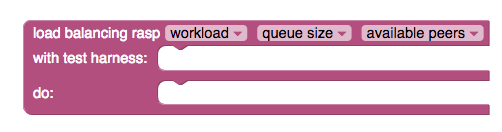
\includegraphics[width=\textwidth]{rasp}
    \caption{\label{fig:rasp}A proposed visual element template for a load
      balancing \rasp in a visual programming language.  Such a \rasp
      would hide the implementation details from students while allowing them
      to provide specific test harnesses to specialize the load balancer
      to the particulars of their programs.}
  \end{minipage}
  \hfill{}
  
\end{figure}

To illustrate our proposed ideas, consider the problem of synthesizing
efficient representations of weighted graphs, as described by Hawkins,
co-PI Fisher and their colleagues~\cite{data-rep-synth}.  Such graphs
consist of a set of vertices, which we assume will be represented
using integers, and a set of edges, which are each defined by a source
vertex, a destination vertex and a weight.  The performance of
standard algorithms, such as forwards and backwards depth-first search
(DFS), will vary substantially depending on the representation of the
edges.  Indeed Hawkins' system considers 68 different representations
of the set of edges as different kinds of hierarchical maps.  Such
maps may be implemented by lists, vectors or hash tables.  And they
may be indexed first by source node, destination node or weight.
Figure~\ref{fig:rep-synth} depicts two plausible
representations.

One way for programmers to describe the space of possible
implementations for sets of edges may be to use data types with
constraints.  For instance, the following definitions coarsely
describe the range of possible representations \cd{R}.

\begin{mylisting}
data Map = List | Hash
data R = Src of Map * R | Dst of Map * R | Pair of (R, R) | Base
\end{mylisting}

Here, a representation \cd{R} may be a \cd{Map} (which may in turn
be a \cd{List} or \cd{Hash} table) indexed by source
or destination vertex, composed with some other (nested) representation
for the rest of the data.  Complex clients may need to access the set of
edges in more than one different way and hence a representation may also
be a \cd{Pair} of representations.

However, not all such representations are reasonable---for instance,
it makes no sense to have a hierarchical structure that includes
maps repeatedly and redundantly indexed by destination (or by source).
A natural way to rule out such structures is to use constraints of
some kind.  We plan to investigate various mechanisms for
expressing such constraints, including GADTs~\cite{gadts},
singleton types~\cite{weirich:singletons} and
liquid types~\cite{liquid-haskell}.

In addition to specifying the possible shapes of data structures,
it is necessary to specify the possible implementations of query
methods.  Such methods should protect clients from having to know
the implementation chosen, and should be as efficient as possible.
We plan to investigate the use of type-directed programming here.
In other words, we plan to allow users to define functions parameterized
by symbolic types; once the symblic types are made concrete, it should
be possible to specialize the function implementation to the chosen
symbolic type without incurring run-time overhead and without giving up
type safety.


%For example, Hancock~\cite{hancock} was ...

%% Accessor methods must be defined so that they traverse the symbolically selected
%% hierarchical structures efficiently and correctly.  Moreover, correct implementations can often only
%% be constructed when the structure satisfy non-trivial representation invariants.  Hence, programmers
%% must be able to define such invariants and the synthesis infrastructure must be able to interpret them.






%% \begin{figure}[t]
%% \centering
%% \begin{mylisting}
%% -- D describes the range of possible implementations
%% data MapType = List | Hash
%% data D =
%%     Base
%%   | SrcKey of MapType * D
%%   | DstKey of MapType * D
%%   | Pair of (D, D)

%% -- good specifies representation invariants
%% good :: Dcomp -> Bool
%% good = ...

%% -- a constrained type that specifies legal representations
%% type GD* :: D where good

%% --
%% query :: GD* -> Query -> Weight

%% -- a symbolic data structure describing
%% symbolic t* :: GD
%% \end{mylisting}
%% \caption{Repesentation synthesis \rasp}
%% \label{fig:rep-synth-rasp}
%% \end{figure}

\section{Evaluation}
\label{sec:eval}

We will evaluate our design ideas using both theoretical machinery and
practical applications.

On the theoretical side, we plan to define the 
static and dynamic semantics of our extensions formally and 
to prove classic type safety theorems to ensure that the interactions
between symbolic types, symbolic values and Haskell's rich type system
do not interfere with one another.  In addition, we plan to study
how symbolic types change or support reasoning principles such as
parametricity, and to investigate logical relations as means
for reasoning about programs in the presence of symbolic types.  
Ahmed's step-indexed logical relations are likely the right place
to begin the investigation.  And to extend the work to stateful programs,
we would consider recent work from Ahmed, Dreyer, Rossberg and others 
as a starting
point~\cite{Ahmed:state-logical-relations,Dreyer:logical-relations}.
Proving safety properties and ensuring established reasoning principles
are available to programmers will help evaluate the meta-theoretic
properties that all programs in our extended language will enjoy.

On the practical side, we plan to use our framework to reimplement
existing stand-alone systems.  We will start by demonstrating we can
reimplement PI Fisher's Autobahn~\cite{autobahn}, Trilla's implicit 
parallelism~\cite{implicit-parallel} and Hawkins (in collaboration with
Fisher again) representation synthesis engine~\cite{implicit-parallel}.  
By reimplementing existing synthesis
systems, we have a baseline against which we can measure the properties
of our new framework, including synthesis time, effort (in terms of lines
of code and person-hours) and performance of the synthesized code.  Naturally,
such measurements will likely inspire further research that aims to
optimize the performance of the framework.   We will also experiment
with and evaluate new search strategies for existing frameworks.  For
example, we are eager to evaluate the tradeoffs in using reinforcement
learn vs genetic programming in applications such Autobahn.

In addition to evaluating the effectiveness of our framework when
re-implementing existing applications, we hope to develop new
applications.  Some of this will be done by mentoring undergraduate
students on independent projects using our new framework.  While it is
difficult to set up a controlled experiment that measures programmer
productivity accurately in this context, we hope to gain ad hoc
insights into the utility of our tools that will lead to their improvement 
through this process.

\section{Broader Impacts}
\label{sec:impact}


% Prose


We will explore using \rasps to enable educators to add new
abstractions to a visual programming language more easily. Visual programming
languages enable students to create software artifacts without
worrying about syntax.
However, As Resnick and Silverman noted after developing the visual language,
Scratch\cite{Scratch}, ``one of the most important
decisions is the choice of the basic building blocks of the
kit. This choice determines, to a large extent, what ideas
users can explore.'' 
To facilitate the construction of blocks,
visual language frameworks, such
as Google's Blockly \cite{Blocks,BlocklyApps}, allow language
developers to
provide a visual front end for an existing textual language.
%In contrast, educators, who typically aren't language developers, 
%want to be able to provide a new high-level
%abstractions for existing visual languages.
As an example of current practice, the visual
language BlockyTalky\cite{BlockyTalky} declares Blockly blocks to wrap distributed
programming primatives while tacitly handling implementation details like establishing
remote connections and buffering message sends in its runtime system.
Researchers have used BlockyTalky to engage middle and high school students
from underrepresented backgrounds in computer science by having them
design their own networked, LEGO, and GrovePi hardware instruments to play music
in summer workshops and music education classrooms.

Educators would find it useful to be able to add higher-level abstractions
to existing visual programming languages, like Scratch or BlockyTalky,
so that students can express more interesting programs quickly.
Unfortunately, adding such features is
difficult at the moment\cite{ScratchExt}. One way is to extend the implementation of
the visual language itself, but that requires the educator to be
intimately familiar with the implementation of the language, which is
not a reasonable requirement.  A second way is to define the new
abstraction in the language itself, but that can be cumbersome using a
visual interface because such abstractions can require a lot of screen
space to express correctly.

We propose to explore how \rasps might allow instructors to use
program synthesis to define new abstractions that take into
consideration details of both the language runtime system and student
programs without having to be intimately familiar with either.  For
example, consider the case where an educator wants to add a load
balancer to their students' toolbox.  The educator might develop a
\rasp such as the one shown in Figure~\ref{fig:rasp} to specify a
widget for spreading messages across a variety of devices that works
even when student programs have very different message sending
properties.

For this part of our project, we will use students from one of
Princeton's independent work seminars (IW) to play the role of
educators building abstractions for a visual programming language.
David Walker will lead one such IW seminar, which will be comprised of 10-15
undergraduate students.  Tufts PhD student Matthew Ahrens, who worked
on BlockTalky, will design and build a \rasp system for the visual
programming language.  The Princeton undergraduates will work together
under the guidance of Professor Walker to build their own \rasp-based
abstractions for a visual language and explore what applications
younger students might be able to build with those abstractions.
As part of the IW seminar, the undergraduates will get exposure to
working on a research project.  They will learn about writing research
proposals, scheduling tasks, planning for contingencies, giving oral
presentations, and writing technical papers.  The seminar provides a
group structure to support the students on their individual research projects.

\section{Collaboration Plan}

PIs Fisher and Walker have been collaborating successfully
with one another for over a decade on projects ranging from the design
and implementation of domain-specific languages for data processing
such as
PADS~\cite{fisher+:next-700,fisher+:pads-overview,mandelbaum:pads-ml}
and Forest~\cite{fisher+:forest} to the development of new algorithms
for program
synthesis~\cite{fisher+:learnpads,miltner+:synthesizing-bijective-lenses,zhu+:learnpads2}.
These colloborations have always occurred with the PIs at separate
institutions, as in the current proposal.  As we have done for our
prior and ongoing collaborations, we will continue to hold weekly
team-wide videoconference meetings.  This mechanism allows everyone to
stay abreast of the activities at both universities and enables all
students to take advantage of the broad knowledge and perspectives
represented across the team.  In this way, the PIs truly co-advise all
graduate students, regardless of their location, which in our
experience produces stronger, higher-impact research.  We also have
frequent email discussions between meetings.  Due to our existing
collaborations we already have a shared Github repository for code,
data, and publications.  We will continue to use this repository to
share and maintain our research artifacts.  The table in
Figure~\ref{fig:timeline} presents a timeline for our collaborative
activities.

\begin{figure}[!hbt]
\begin{small}
\centering
\begin{tabular}{|l|c|c|}
\hline\hline
{\bf Research Task} & {\bf Start} & {\bf Finish} \\
\hline\hline
Control Structure Synthesis Infrastructure & Year 1 & Year 1\\\hline
Control Structure Applications  & Year 1& Year 1 \\\hline
Representation Synthesis Infrastructure & Year 2 & Year 2\\\hline
Representation Synthesis Applications  & Year 2 & Year 2\\\hline\hline
{\bf Educational Task} & {\bf Start} & {\bf Finish} \\\hline\hline
Blockly Infrastructure Development & Year 1 & Year 2 (Fall) \\\hline
Princeton UGrad IW Seminar & Year 2 (Spring) & Year 2 (Spring) \\\hline\hline
\end{tabular}
\end{small}
\caption{Research Timeline}\label{fig:timeline}
\end{figure} 

\section{Results from Prior NSF Support}
\label{sec:prior-support}

\noindent
{\bf Kathleen Fisher} has not applied for nor received funding from NSF in the past
five years.

\medskip

\noindent
{\bf David Walker, PI. NSF CNS-1111520, Intellectual Merit:}
In NSF CNS-1111520, \emph{High-Level Language Support for Trustworthy Networks}
(\$1,400,000, 08/11-07/16),
PI Walker and his collaborators developed new languages, interfaces
and systems for managing software-defined networks (SDNs).
This project produced the Frenetic family
of network programming languages, the first high-level languages for
programming software-defined networks.  These languages, which include
Frenetic~\cite{frenetic},
Pyretic~\cite{pyretic},
NetKAT~\cite{netkat} and others, all adhere to the
\emph{principle of compositionality}, a key design element missing
from earlier network programming languages.
%They also invented the
%notion of consistent network update~\cite{reitblatt+:consistent-updates},
%which ensures key safety invariants are preserved across network update.
Open source code for systems produced by this project is available
at \url{frenetic-lang.org}.
%
{\bf Broader Impacts:}
The PIs held a well-attended summer school on network programming and
verification for students and faculty. The
Pyretic programming language was used in Nick Feamster's popular
SDN MOOC; thousands of students and
network operators all over the US used it to learn principles of network
programming.  The PIs
also helped create the P4 switch configuration language~\cite{P4}, which is
becoming an industry standard.

\noindent
{\bf David Walker, PI. NSF CNS-1703493, Intellectual Merit:}
All sectors of society depend upon properly functioning networks, and
yet network configuration today is highly error-prone.  Such misconfigurations
can and do lead to network downtime that can take critical systems off-line
and cost companies or the government millions in lost revenues.
In NSF CNS-1703493, \emph{NeTS: Medium: Collaborative Research: Network Configuration Synthesis: A Path to Practical Deployment}
(\$423,891 (Princeton portion), 07/17-06/21), we plan to build on work on network configuration
synthesis and verification.  By synthesizing network configurations from
high-level specifications, we can avoid entire classes of bugs; by applying
verification technology to synthesized or legacy configurations, we can
root out additional errors.  Though this grant has just begun, we have already
made substantial progress by showing how to scale synthesis of network configurations to networks with hundreds or thousands of routers using abstract topologies~\cite{propane-at}.  We also designed, implemented and optimized a new
network verification tool that translates configurations for OSPF, BGP and
other standard protocols into SMT formulas for verification of a wide range
of properties ranging from reachability to fault tolerance to multi-path
consistency~\cite{minesweeper}.  Both systems are available open source
on github (\url{https://github.com/rabeckett/propane} and \url{https://batfish.github.io/minesweeper/}).
{\bf Broader Impacts:} The Propane system is currently being used in
colleague Jennifer Rexford's graduate networking class to teach the basics
of network configuration and analysis.  The PIs will host
a workshop on network synthesis and verification under the umbrella of the
Cornell-Princeton Center on Network Programming and with ample industry
participation as a way of transferring academic discoveries to industry.




%%% Local Variables:
%%% mode: latex
%%% TeX-master: "proposal.tex"
%%% TeX-PDF-mode: t
%%% End:
